\chapter{Experimental Results}
\label{chapter6}
\thispagestyle{empty}

\begin{quotation}
{\footnotesize
\noindent\emph{``Quote 6''}
\begin{flushright}
Author 6
\end{flushright}
}
\end{quotation}

\vspace{0.5cm}

%\noindent Si mostra il progetto dal punto di vista sperimentale, le cose materialmente realizzate. In questa sezione si mostrano le attivit\`a sperimentali svolte, si illustra il funzionamento del sistema (a grandi linee) e si spiegano i risultati ottenuti con la loro valutazione critica. Bisogna introdurre dati sulla complessit\`a degli algoritmi e valutare l'efficienza del sistema.

\section{Accuracy of the Detection Algorithm}

\vspace{0.5cm}

\section{Experiments}

Here we describe the set of experiments that we run on the dataset. Each experiment has been executed classifying data with a Random Forest classifier and
a Support Vector Machine.

\vspace{0.5cm}

\subsection{Normalization}

Te first aspect that we took into account regarded \textit{normalization} of data. Each feature in the \textit{feature vector} can range among different values.
The procedure described in the guide in \cite{SVM01} claims that the scaling of data is very important in order to obtain a good classification with \Glspl{SVM} \cite{juszczak2002feature}.
On the other hand, \Glspl{RF}, as composed of \Glspl{DT}, should not be influenced by scaling.\\
The general idea is to rescale the data so that each new feature \textit{z} has: $\mu = 0, \sigma = 1$, using the following relations:

\begin{eqnarray}
 \mu & = \frac{1}{N} & \sum_{i=1}^{N} x_i \\
 \sigma & = & \sqrt{ \frac{1}{N} \cdot \sum_{i=1}^{N}(x_i - \mu)^2 } \\
 z_i & = & \frac{x_i - \mu}{\sigma}
\end{eqnarray}

We run some test with different sets of features.
\\
The Matlab code implemented to run \textit{experiment 1} is listed in \ref{appendixB:exp1}

\vspace{0.5cm}

\subsection{Extended Dataset}

We analyzed the effect of considering the extended dataset, as described in Section \ref{ch4:ed}. Rotated and mirrored images should provide some information for
all the features that are orientation dependent, in all the other cases, the added elements are just replicates of already present instances.
Also in this case we run test with different sets of features.
\\
The Matlab code implemented to run \textit{experiment 2} is listed in \ref{appendixB:exp2}


\vspace{0.5cm}

\subsection{Best Features Combinations}

In this experiment we looked for the best combination of features, so we considered all the features described in \ref{ch4:FE}. Having \textit{n} features, maybe multi-component,
they can be combined in $2^n-1$ ways. As the texture features (see Section \ref{ch4:tf}, in particular Equation \ref{ch4:tftypes}) are mutually exclusive, we run three different
experiment, one for each texture feature set.
\\
The Matlab code implemented to run \textit{experiment 3} is listed in \ref{appendixB:exp3}

\vspace{0.5cm}

\subsection{Dataset Dimension}

In this experiment we analyzed the effect of the size of the training dataset on the classification performance. To achieve this goal, we repeatedly selected random subsets of the
extended dataset and applied our classifier. To avoid the dependence on the specific selected subset, we run many different experiments with randomly chosen subsets with the same 
size and then we averaged the results.
\\
The Matlab code implemented to run \textit{experiment 4} is listed in \ref{appendixB:exp4}

\vspace{0.5cm}

\subsection{SVM parameters}

In the experiments above we noted that \Glspl{SVM} are more sensible to the selected features and to the size of the dataset, meaning that, in some cases, \Gls{SVM} performs poorly on data.
So we decided to analyze in a deeper way if some of the configuration options of the classifier (i.e. kernel type [Section \ref{ch4:svm}], degree in kernel function, etc. ) could improve the performance.
\\
The Matlab code implemented to run \textit{experiment 5} is listed in \ref{appendixB:exp5}

\vspace{0.5cm}


\subsection{Principal Component Analysis}

Even when considering only simple features, the feature space can reach high dimensions (i.e. a lot of components). It is common experience,
in many classification problems, that when the dimensionality increases, the volume of the space increases so fast that the meaningful data become sparse
in a substrate of noise.\\
This situation is often referred to as the \textit{curse of dimensionality} \cite{bellmandynamic}.
In \Gls{ML} problems that involve learning from a finite number of data samples in a high-dimensional feature space,
with each feature having a number of possible values, an enormous amount of training data are required to ensure that there are several samples with each combination of values.
With a fixed number of training samples, the predictive power reduces as the dimensionality increases, and this is known as the \textit{Hughes effect} \cite{hughes}.\\
\Gls{PCA} is a way to reduce the dimensionality of the dataset \cite{PCA_jolliffe}. \Gls{PCA} is a mathematical procedure that uses an orthogonal transformation
(SVD transformation) to convert a set of observations of possibly correlated variables into a set of values of linearly uncorrelated variables called \textit{principal components}.
This transformation is defined in such a way that the components are sorted in descending magnitude of \textit{explained variance}: that is, the first principal component
has the largest possible variance ( accounts for as much of the variability in the data as possible), and each succeeding component, has the highest variance possible under the constraint
that it is orthogonal to (i.e., uncorrelated with) the preceding components. \Gls{PCA} is sensitive to the relative scaling of the original variables, 
and so we applied it on normalized data \cite{PCA02_applications}.
In our experiments we selected some datasets with high dimension feature spaces, applied \Gls{PCA} and classified the resulting components adding one component at a time, with the aim to
observe the classification performances in relation to the number of components and the percentage of explained variance.
\\
The Matlab code implemented to run \textit{experiment 6} is listed in \ref{appendixB:exp6}


\vspace{0.5cm}

\subsection{Size of the Image Patch}

In all the experiments above, we considered the size of each image patch, on which to compute features, to be $100\times100$ pixels.
We wanted to analyze if there is a smaller sub-image that includes all the meaningful information, while the boundary contains essentially background (i.e. noise for the
purposes of classification), while an excessively small patch would not allow to classify data.\\
So we run experiments considering, form time to time, bigger portions of the images and analyzed the classification performances.
\\
The Matlab code implemented to run \textit{experiment 7} is listed in \ref{appendixB:exp7}



\vspace{0.5cm}





\section{Accuracy of Humans}

\vspace{0.5cm}

\section{Accuracy of Algorithms}

(rif. paper)

\subsection{Performances of Algorithms on MITOS Dataset}
\label{ch6:icpr_perf}

We report here the performances of the best-scoring algorithms that participated to the ICPR2012 Contest, as shown on the contest website (Figure \ref{ch6:fig3}).
The principal metric adopted to compare algorithms is the $F_1$-Score (Figure \ref{ch6:fig3:a}) , but also precision and recall are shown \ref{ch6:fig3:b}. 

\begin{figure}[!htb]
  \centering
    \subfigure[F-Score]{
      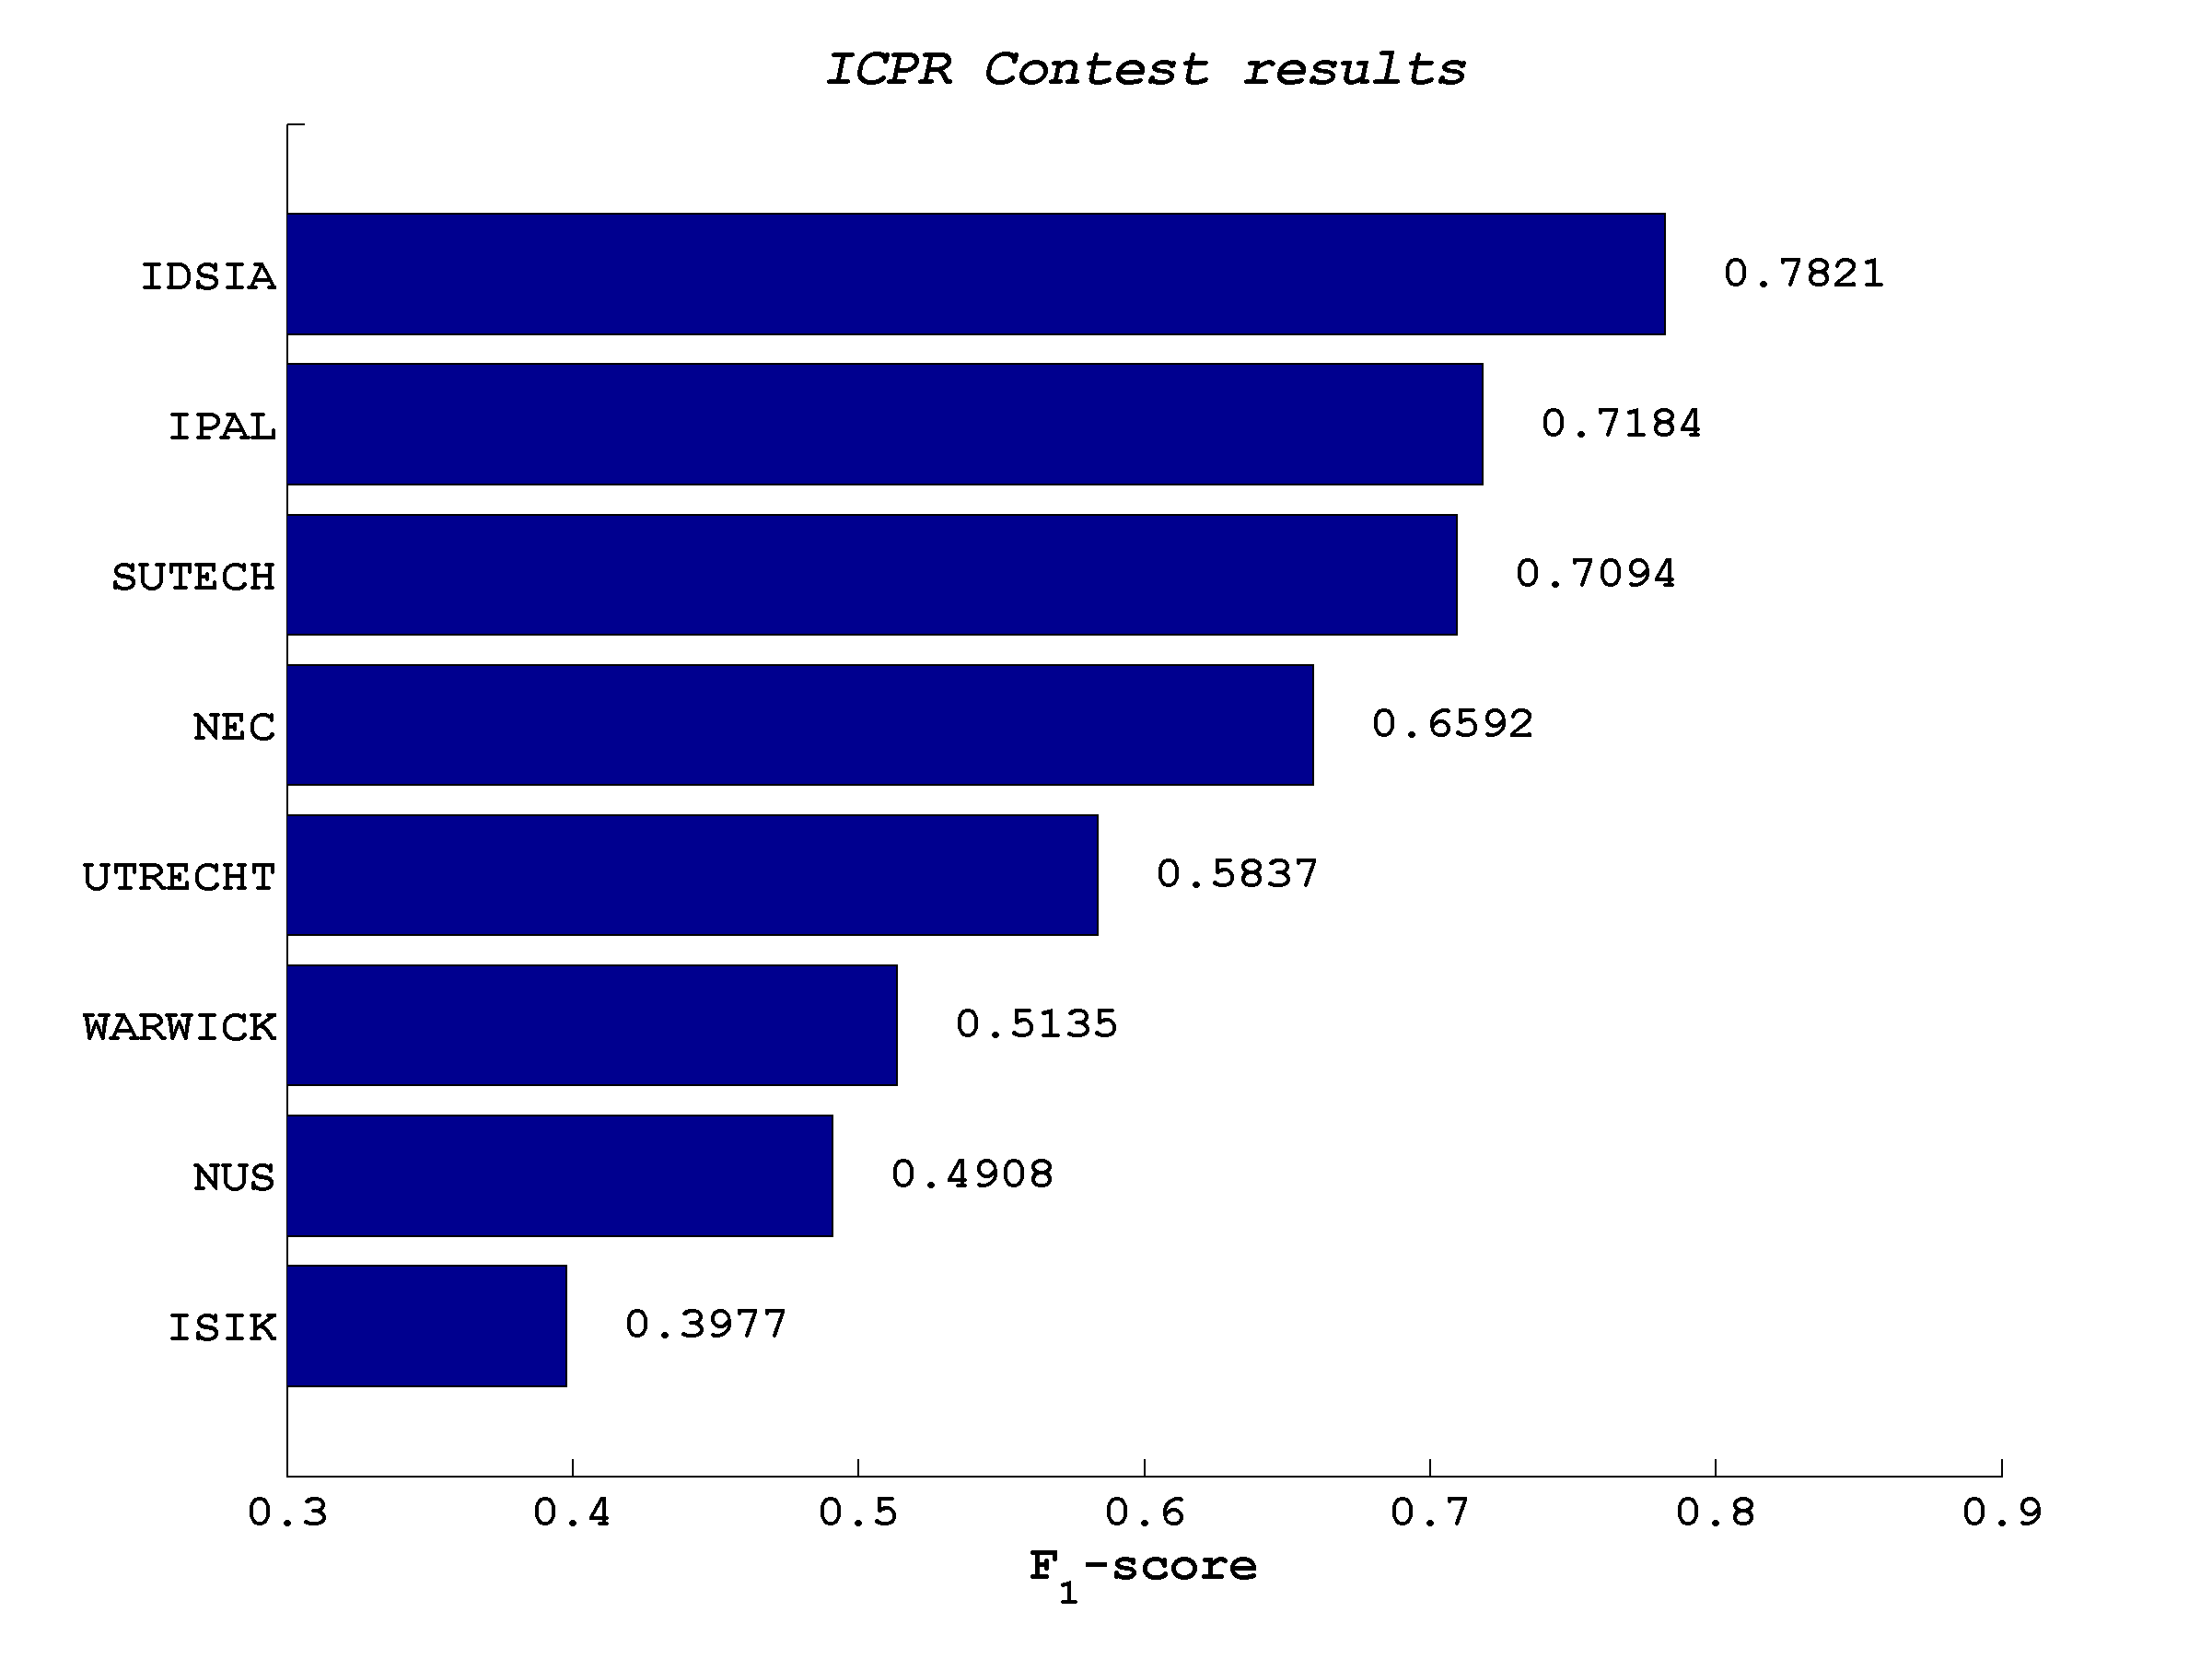
\includegraphics[width=0.82\textwidth]{./images/ICPRperf1.png}
      \label{ch6:fig3:a}
    }\\
    %\hspace{1mm}
    \subfigure[metrics]{
      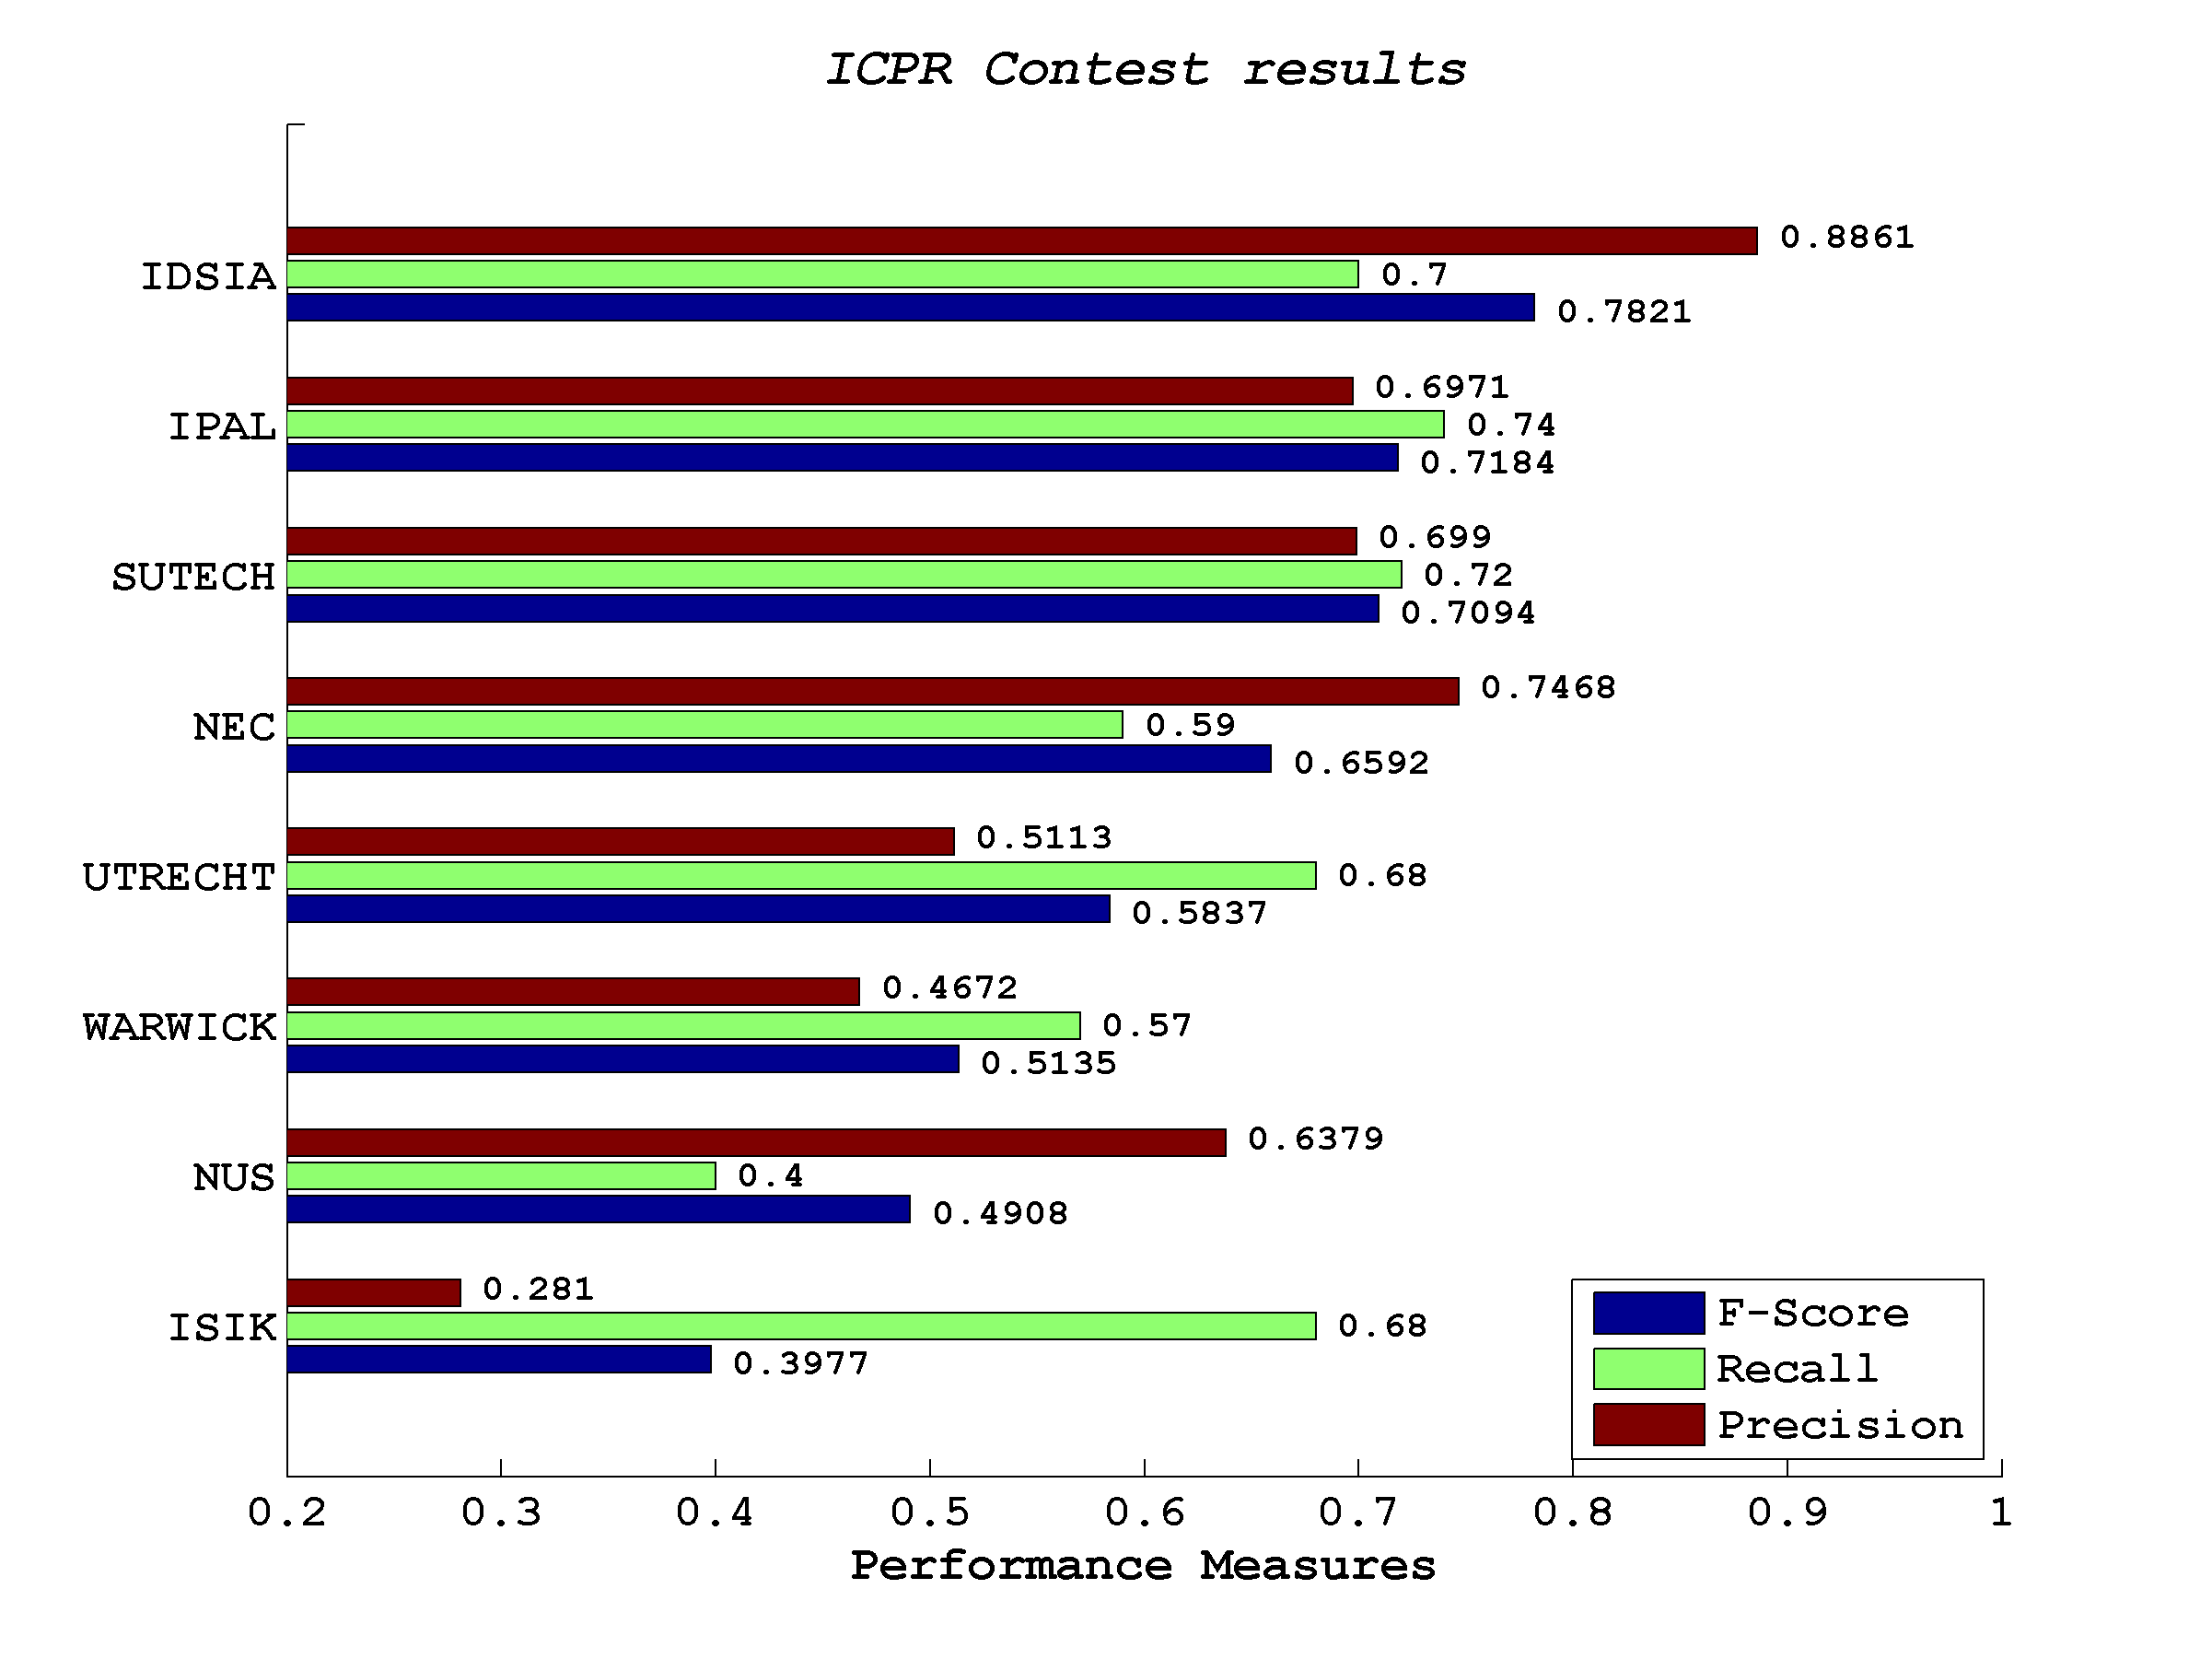
\includegraphics[width=0.82\textwidth]{./images/ICPRperf2.png}
      \label{ch6:fig3:b}
    }
    \caption{Performances of best algorithms in ICPR 2012 contest}
    \label{ch6:fig3}
\end{figure}